\newpage


\section{Tour / examples}
\label{sec:tour}

Next, we will walk through a series of examples, in varying level of complexity. Each example will demonstrate different aspects of serializable vs non-serializable programs.
%
The first examples are relatively basic, while the last examples have higher complexity and are motivated by real word problems, e.g., BGP routing policy updates.
%
Global variables are depicted with upper-case characters, while local variables (per each request) are depicted with lower-case ones.
%
Unless explicitly state otherwise, all global and local variables are initialized to 0.
%
The ``\textit{?}'' symbol depicts a nondeterministic choice between ``0'' and ``1''. All other constructs (\textit{while}, \textit{yield} \textit{if}) have their common interpretation.

\guy{Is the above paragraph clear?}

\subsection{Example 1}

%\subsubsection{Example 1}

We start with a basic example, describing a single request {\color{ForestGreen}$\blacklozenge_\text{A}$}, a single local variable (``x'') per each request; and a single global variable (``FLAG'') shared among all in-flight requests. 
%
In Listing~\ref{lst:BasicSer} an in-flight request assigns to x the value of FLAG (hence, initially, [$x:=0$]). Then, the request non-deterministically chooses whether to yield, or to flip the value of $x$. Subsequently, FLAG is assigned 1 and the value of x is returned as the response to request {\color{ForestGreen}$\blacklozenge_\text{A}$}. 
%
Note that the presence of the \textit{else} branch renders the program serializable, as intuitively, the returned value of x does not depend on the assignment of FLAG.
%
However, this changes in  Listing~\ref{lst:BasicNonSer}. In which case there is no ``else'' branch and x is always assigned the value of FLAG.
%
It is straightforward to see that this update makes the program non-serializable. Any serial execution will afford the first request {\color{ForestGreen}$\blacklozenge_\text{A}$} the matching returned response {\color{red}$\blacklozenge_0$} (as $[x:=FLAG]$, which is initially 0). As the first request also assigns $[FLAG:=1]$ before exiting, any subsequent execution will assign $[x:=1]$ and hence return the response {\color{red}$\blacklozenge_1$}. Differently put, for any serial execution with i requests --- we have exactly one (first) request/response pair {\color{ForestGreen}$\blacklozenge_\text{A}$}/{\color{red}$\blacklozenge_0$}, and $(i-1)$ pairs of {\color{ForestGreen}$\blacklozenge_\text{A}$}/{\color{red}$\blacklozenge_1$}.
%
However, given that the first request can also \textit{yield}, it is possible for another request to subsequently run the program after the first request yields and before it returns. This, in turn, will allow two requests to have $[x=0]$, and hence, any number of arbitrary requests can have multiple {\color{ForestGreen}$\blacklozenge_\text{A}$}/{\color{red}$\blacklozenge_0$} pairs. Thus, Listing~\ref{lst:BasicNonSer} is not serializable.




%\vspace{2em}
%example - 2

% Second row
\noindent
\begin{minipage}[t]{0.45\textwidth}
	\begin{lstlisting}[caption={Serializable},
		label={lst:BasicSer}]
	request A: 
		x := FLAG
		
		if (?):
			yield
		else:
			x := 1 - x
		
		FLAG := 1
		return x
	\end{lstlisting}
\end{minipage}
\hfill
\begin{minipage}[t]{0.45\textwidth}
	\begin{lstlisting}[caption={Not serializable: {(A,0),(A,0)}},
	label={lst:BasicNonSer}]
			request A: 
			    x := FLAG 
			
			    if (?): 
			        yield
			    // no else
			
			
			    FLAG := 1 
			    return x
		\end{lstlisting}
\end{minipage}%

\subsection{Example 2}

%\subsubsection{Example 2}
The following program pairs have a single global variable ``X'', and two requests --- {\color{ForestGreen}$\blacklozenge_\text{incr}$} which increments X by 1, and {\color{ForestGreen}$\blacklozenge_\text{decr}$} which decrements X by 1. Both program have while loops which guarantee that X will always be assigned a value between 0 to 3, otherwise the while loop will yield an infinitum. Both requests return the value of X after updating it.
%
In the first case, Listing~\ref{lst:FredSer} presents a serializable execution, due to the absence of any yield between the increment/decrement of X, and its return. Equivalently, in each of the requests, the update of X and the returned value can be thought of as \textit{a single atomic execution}.
%
However, in Listing~\ref{lst:FredNonSer},we add an additional yield (and a local variable ``y''), occurring in each of the requests, between the update of X and it's return.
%
This updates allows request of the same type to update X to the same value --- something that is not possible in any serial execution. 

%\vspace{2em}
%\newpage
%example - 3

% Third row
\noindent
\begin{minipage}[t]{0.45\textwidth}
	\begin{lstlisting}[caption={Fred (serializable)},
		label={lst:FredSer}]
			request incr: 
			    while (X == 3):
			        yield
			        
			        
			    X := X + 1
				  return X		
			
			request decr: 
			    while (X == 0): 
			        yield
			        
			        
			    X := X - 1
				  return X
		\end{lstlisting}
\end{minipage}
\hfill
\begin{minipage}[t]{0.45\textwidth}
	\begin{lstlisting}[caption={Fred2 (not serializable)},
		label={lst:FredNonSer}]
			request incr:
			    while (X == 3):
			        yield
			    y := X
			    yield
			    X := y + 1
		      return X		
			
			request decr: 
			    while (X == 0):
			        yield
			    y := X
			    yield
			    X := y - 1
		      return X
		\end{lstlisting}
\end{minipage}
	
\subsection{Example 3}
%\subsubsection{Example 3}	
%\todo{continue}	
%example - 6

The next pair of examples cover a setting in which there is a single global variable (X) and a single local variable per each in-flight request. The {\color{ForestGreen}$\blacklozenge_\text{flip}$} requests flips the bit of the single initial variable X (initialized to 0); the {\color{ForestGreen}$\blacklozenge_\text{main}$} request attempts to decrement i five times.
%
It is straightforward to observe that the program in Listing~\ref{lst:ComplexWhileSer} is trivially serializable, as there are no yields.
%
However, by adding the two yields and updating the program (see Listing~\ref{lst:ComplexWhileNonSer}) it becomes non-serializable. This can be observed as follows --- given a single in-flight request, the value of X is either 0 or 1, and hence, exactly one of the while loops will run indefinitely. Thus, any serializable execution will result into a set without any {\color{ForestGreen}$\blacklozenge_\text{main}$}/{\color{red}$\blacklozenge_1$} pairs, but rather only, perhaps terminating {\color{ForestGreen}$\blacklozenge_\text{flip}$} requests.
%
However, given at least $i=5$ interleaving of in-flight {\color{ForestGreen}$\blacklozenge_\text{flip}$} requests, it is possible for a {\color{ForestGreen}$\blacklozenge_\text{main}$} request to terminate and bypass all while loops, something that cannot occur in serializable executions.


% Second row
\noindent
\begin{minipage}[t]{0.45\textwidth}
	\begin{lstlisting}[caption={Complex while (serializable)},
		label={lst:ComplexWhileSer}]
		    request flip: 
		        X := 1 - X 
		    
		    request main:
		        i := 5
		        while (i > 0):
		            while (X == 0):
		                pass
		            while (X == 1):
		                pass
		            i := i - 1
		        
		        return 1       
				\end{lstlisting}
\end{minipage}%
\hfill
\begin{minipage}[t]{0.45\textwidth}
	\begin{lstlisting}[caption={Complex while with yields (not serializable)},
		label={lst:ComplexWhileNonSer}]
		    request flip: 
		        X := 1 - X 
		
		    request main:
		        i := 5
		        while (i > 0):
		            while (X == 0):
		                yield
		            while (X == 1):
		                yield
		            i := i - 1
		
		        return 1        
					\end{lstlisting}
\end{minipage}
	
	
	
\subsection{Example 4}
%\subsubsection{Example 4: Banking System}

The next example emulates a simple banking system, as motivated by Chandy and Lamport's seminal paper~\cite{ChLa85}. The system operates on two accounts of the same user --- denoted with the global variables $A$ and $B$, and initialized to have $100\$$ and $50\$$ respectively. 
%
Each {\color{ForestGreen}$\blacklozenge_\text{transfer}$} request allocates $50\$$ from account $A$ to account $B$, and every {\color{ForestGreen}$\blacklozenge_\text{interest}$} request adds $t\%$ interest to each account. For simplicity, and without loss of generality, we chose $t=100\%$, hence doubling the funds in each account, per each such request. We also note that for simplicity we depict two accounts ($A$ and $B$), although this example is valid for any number of accounts.
%
Both requests return the sum of final client funds in both the accounts.  
%
Listing~\ref{lst:BankSer} depicts a serializable version of this banking system (without any yields), while Listing~\ref{lst:BankNonSer} includes yields in each of the requests, between the adjustment of accounts $A$ and $B$ (we note that this also represents real world systems in which the account can be sharded and partitioned across different nodes).
%


\noindent
\begin{minipage}[t]{0.45\textwidth}
	\begin{lstlisting}[caption={bank (serializable)},
		label={lst:BankSer}]
	    // initialize accounts
	    A := 100
	    B := 50
	    
	    request transfer: 
	        // transfer 50$
	        A := A - 50
	        // no yield
	        B := B + 50
	        return A + B
				
	    request interest: 
	        // add a 100% interest
	        A := A + A
	        // no yield
	        B := B + B
	        return A + B	      		        
			\end{lstlisting}
\end{minipage}
\hfill
\begin{minipage}[t]{0.45\textwidth}
	\begin{lstlisting}[caption={bank with yields (non serializable)},
		label={lst:BankNonSer}]
	    // initialize accounts
	    A := 100
	    B := 50
			
	    request transfer: 
	        // transfer 50$
	        A := A - 50
	        yield
	        B := B + 50
	        return A + B
	
	    request interest: 
	        // add a 100% interest
	        A := A + A
	        yield
	        B := B + B
	        return A + B	      		        
		\end{lstlisting}
\end{minipage}
	

Interestingly, in this setting, serializability also corresponds to correctness invariants pertaining to the program. Specifically, in every serializable execution, it holds that for $A_{\textit{before}},B_{\textit{before}}$ marking the funds before running a single {\color{ForestGreen}$\blacklozenge_\text{interest}$} request, and any number of {\color{ForestGreen}$\blacklozenge_\text{transfer}$} requests (and $A_{\textit{after}},B_{\textit{after}}$ marking the corresponding state after those requests), then:
\[
\bigl(A_{\mathit{after}} + B_{\mathit{after}}\bigr)
= (1 + t\%)\,\bigl(A_{\mathit{before}} + B_{\mathit{before}}\bigr).
\]

This invariant always holds for any such serial execution, while having the specific division \textit{between} accounts $A$ and $B$ depending on the actual order of the serial execution.
%
However, this correctness invariant does not hold for non serializable executions. For example, in a setting in which there is a single {\color{ForestGreen}$\blacklozenge_\text{transfer}$} request, which deduces $50\%$ from account $A$, and then yields (resulting to a temporary state in which $[A=50\$,B=50\$]$); subsequently followed by an  {\color{ForestGreen}$\blacklozenge_\text{interest}$} request which runs until completion, in which case  $[A=100\$,B=100\$]$, and then, the remainder of the yielded {\color{ForestGreen}$\blacklozenge_\text{transfer}$} request is executed, resulting finally to $[A=100\$, B=150\$]$.  This result in $50\$$ ``missing'' from our system, due to this non serializable behavior.
%
As mentioned, a serial execution of a these two request will always result to 
$A+B=2\cdot (100\$+50\$)=300\$$, with either a final state of $[A=150\$, B=150\$]$ or $[A=100\$, B=200\$]$, depending on the scheduled serializable order.




%\newpage
\subsection{Example 5}

The following example motivates our routing‐policy programs in software‐defined networking (SDN). In SDN, switches not only forward packets but can also be programmed in domain‐specific languages (e.g., P4). At runtime, a centralized controller node can adjust the global network control policy. The controller can also periodically send control packets to each switch, causing it to adopt its updated routing as dictated by the updates.
%
An instance of a simple network with two competing policies is shown in Fig.~\ref{fig:BgpRoutingPolicies}. This network consists of four nodes (numbered 0 through 3), with the two middle nodes --- node 1 (labeled \textit{WEST}) and node 2 (labeled \textit{EAST}), serving as ingress points from where traffic may nondeterministically enter the network. The controller selects one of two policies: a \textcolor{ForestGreen}{green} policy, which routes traffic from West to East, or a \textcolor{red}{red} policy, which routes it in the opposite direction.


%// [WEST, switch 1] ---> [EAST, switch 2] ---> [out, switch 3] 
%else:
%G := 0 // red policy
%// [out, switch 0] <--- [WEST, switch 1] <--- [EAST, switch 2] 



\begin{figure}[H]
	\centering
	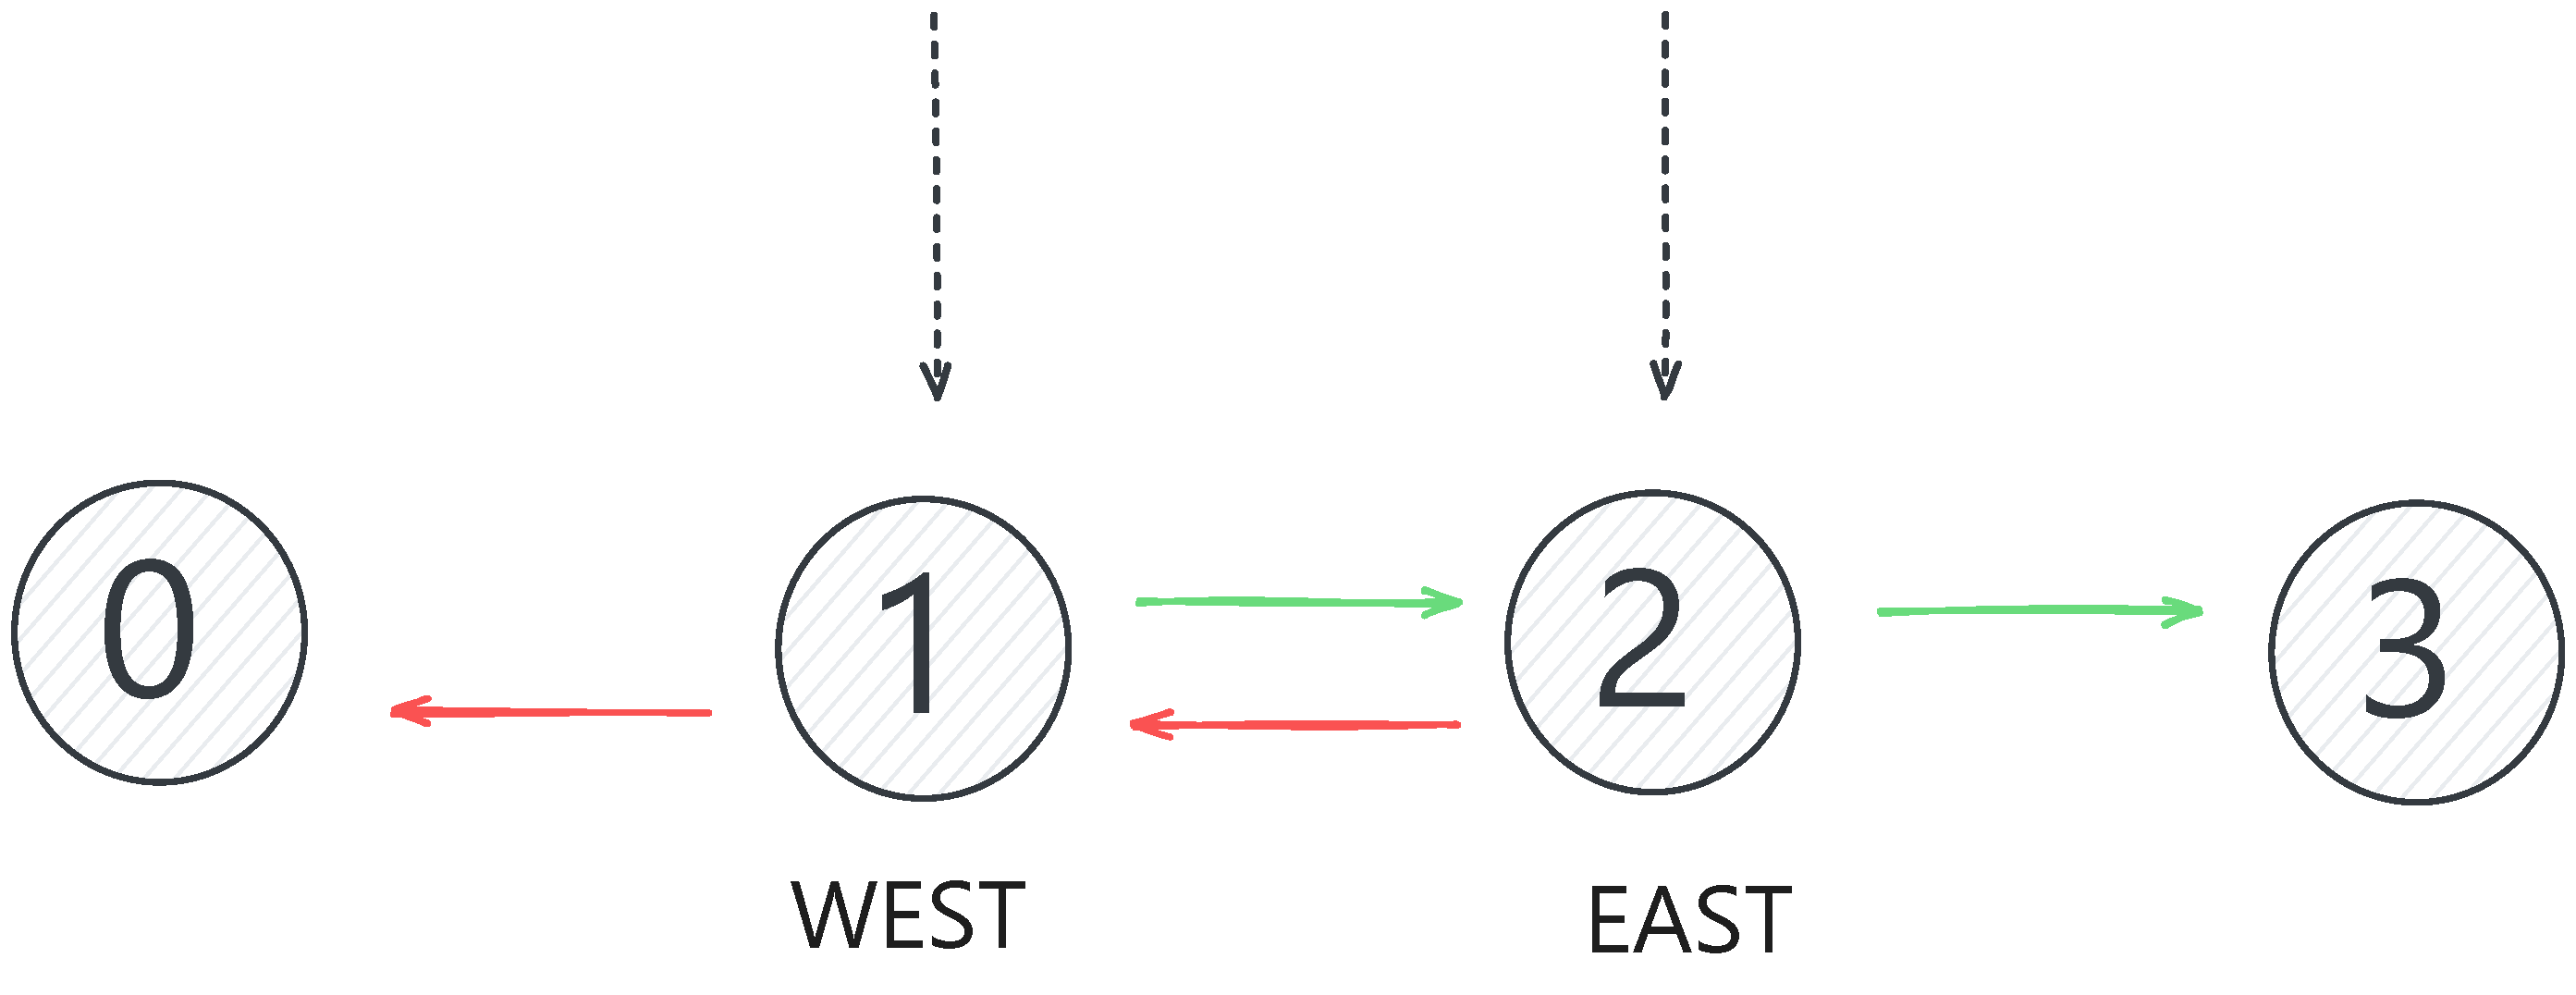
\includegraphics[width=0.7\linewidth]{plots/east_west_routing.pdf}
	\caption{Routing policy in example 5.}
	\label{fig:BgpRoutingPolicies}
\end{figure}

This SDN-controlled routing policy is realized in the pseudo code in Listing~\ref{lst:BgpNonSerializable}.
%
The program includes a single global variable $G$, indicating if the current routing policy is the  \textcolor{ForestGreen}{green} policy ($[G=1]$) or the \textcolor{red}{red} policy ($[G=0]$).
%
The program has three types of requests:
\begin{itemize}
	
	\item
	{\color{ForestGreen}$\blacklozenge_\text{policy update}$}:
%	\textit{policy update}:
 represents a controller  update, which nondeterministically decides whether to update the policy (i.e., flip the value of  variable $G$) or not.
	
		\item
	{\color{ForestGreen}$\blacklozenge_\text{route\_from\_west}$}:
	 this request represents a packet entering the network from the \textit{WEST} node (node 1).
	
		\item
{\color{ForestGreen}$\blacklozenge_\text{route\_from\_east}$}: this request represents a packet entering the network from the \textit{EAST} node (node 2).
	
\end{itemize}


Each of the routing requests represents a single packet entering the network. The request includes a local \textit{current} variable representing the index of the current node visited. This variable is initialized as the ingress node value, and updated to emulate the chosen routing path. There is also a \textit{visited\_east} variable (or a \textit{visited\_west} variable, depending on the request in question).
%
The return value of the {\color{ForestGreen}$\blacklozenge_\text{route\_from\_west}$} requests is the sum \textit{(current+current+visited\_east)}. This is an identifier encoding all possible \textit{(current\_switch, visited\_east)} pairs.
%
The program is not serializable, as witnessed by an interleaving that can give rise to final return value of \textit{(current+current+visited\_east)=1} (due to \textit{current=0} and \textit{visited\_east=1}). This represents a routing cycle in the network, which is possible only when updated the routing policy after a request has already been routed based on the previous policy.
Legal, acyclic routes of this request have either a return value of 0 (in the case of [\textit{current=0}, \textit{visited\_east=0}]) or 7 (in the case of [\textit{current=3}, \textit{visited\_east=1}]).
Potential routing cycles can also be observed via non serializable executions also for the  {\color{ForestGreen}$\blacklozenge_\text{route\_from\_east}$} requests.



\begin{minipage}[t]{1.0\textwidth}
	\begin{lstlisting}[caption={BGP (non serializable --- cycles can appear)},label={lst:BgpNonSerializable}]
	    // initialize accounts
	    G := 0
	    
	    request policy_update:
	    if (?):
	        G := 1  // green policy 
	    else:
	        G := 0 // red policy
			
	    request route_from_west:
	        visited_east := 0
	        current := 1
	        while (current == 2) or (current == 3): // still routing        
	            if (current == 1): // west (switch 1)
	                if (G == 1): // green policy
	                    current := 2
	                else: // red policy
	                    current := 1
	            if (current == 2): // east (switch 2)
	                visited_east := 1
	                if (G == 1): // green policy
	                    current := 3
	                else: // red policy
	                    current := 1
	 
	            yield
			
	        return current + current + visited_east
	        
	    request route_from_east:
	        ... // dual case     		        
		\end{lstlisting}
\end{minipage}






\subsection{Example 6}

\guy{suddenly I'm not so sure about this example. It is indeed sound but maybe a bit silly?}


The next program is motivated by system monitoring.
The system has two nodes (represented by the global variables $N_1$ and $N_2$) which monitor ongoing traffic in the network, and are originally both active (as indicated by their initial values [$N_1=1,N_2=1$]).
%
The {\color{ForestGreen}$\blacklozenge_\text{main}$} request takes a ``snapshot'' of the system, i.e., locally records the current activation status of each of the two nodes.
%
Subsequently, in the first request, and any future ones in which both nodes are active, each in-flight request thread  non-deterministically decides which of the two nodes to deactivate, i.e. set [$N_i:=0$]. This policy is consistent with real-world settings for maintaining overall energy efficiency.
%
The {\color{ForestGreen}$\blacklozenge_\text{main}$} request eventually returns the current sum of active nodes in the system.
%
In order for the system to emulate multiple iterations, our setting also includes two additional requests, {\color{ForestGreen}$\blacklozenge_\text{activate\_n1}$},{\color{ForestGreen}$\blacklozenge_\text{activate\_n2}$} which activate the nodes $N_1$ and $N_2$, respectively.
%
We note that the program is non-serializable due to the yield operation that appears immediately after the recording (snapshot) of the node activity. One such example for a non-serializable behavior occurs when two {\color{ForestGreen}$\blacklozenge_\text{main}$} requests record two active monitor nodes and yield; Then, having each request turn off the complement node. As a result of each request operating based on its isolated ``snapshot'' of the initial global state, both monitor nodes can be turned off and we can attain a request with {\color{ForestGreen}$\blacklozenge_\text{main}$}/{\color{red}$\blacklozenge_0$} (for [$N_1+N_2=0+0=0$]).
%
We note that in any serializable execution, no two {\color{ForestGreen}$\blacklozenge_\text{main}$} requests can record both monitors as active, and hence, they cannot both have an interleaving in which each separate monitor is deactivated (hence, a response of {\color{red}$\blacklozenge_0$} is unattainable in serializable executions).




\begin{minipage}[t]{1.0\textwidth}
	\begin{lstlisting}[caption={Snapshot-based monitor deactivation (not serializable, as it can return a sum of 0 active monitors)}]
			// initialize both monitors to be active
			N_1_ACTIVE := 1
			N_2_ACTIVE := 1
			
			request main:
				// take snapshot
				n_1_active_snapshot := N_1_ACTIVE
				n_2_active_snapshot := N_2_ACTIVE
				yield
				
				if (n_1_active_snapshot == 1) and (n_2_active_snapshot == 1):
				// if both nodes active --- choose which one to deactivate 
					if (?): 
						  N_1_ACTIVE := 0
					else:
						  N_2_ACTIVE := 0
					
				return N_1_ACTIVE + N_2_ACTIVE  // total active nodes
				
			
			request activate_n1:
				    N_1_ACTIVE := 1
			
			request activate_n2:
				    N_2_ACTIVE := 1
			
			
		\end{lstlisting}
\end{minipage}

%only 0 in non-serializable runs!

%\todo{start}

%/snapshot_isolation_directly_as_NS_with_yields

%\begin{figure}[h]
%	\centering
%	\includegraphics[width=1.0\linewidth]{plots/snapshot\_isolation\_JSON\_with\_yields.pdf}
%	\caption{Snapshot Isolation with Yields.}
%	\label{fig:snapshotIsolationJsonWithYields}
%\end{figure}
%
%
%
%%/snapshot_isolation_directly_as_NS_without_yields
%
%\begin{figure}[h]
%	\centering
%	\includegraphics[width=1.0\linewidth]{plots/snapshot\_isolation\_JSON\_without\_yields.pdf}
%	\caption{Snapshot Isolation without Yields.}
%	\label{fig:snapshotIsolationJsonWithoutYields}
%\end{figure}


%\todo{maybe we have: (1) a copy of the global automaton; (2) a copy of the local automaton (with yields) with coloring of edges that don't exist in the one without yields}


%\begin{figure}[h]
%	\centering
%	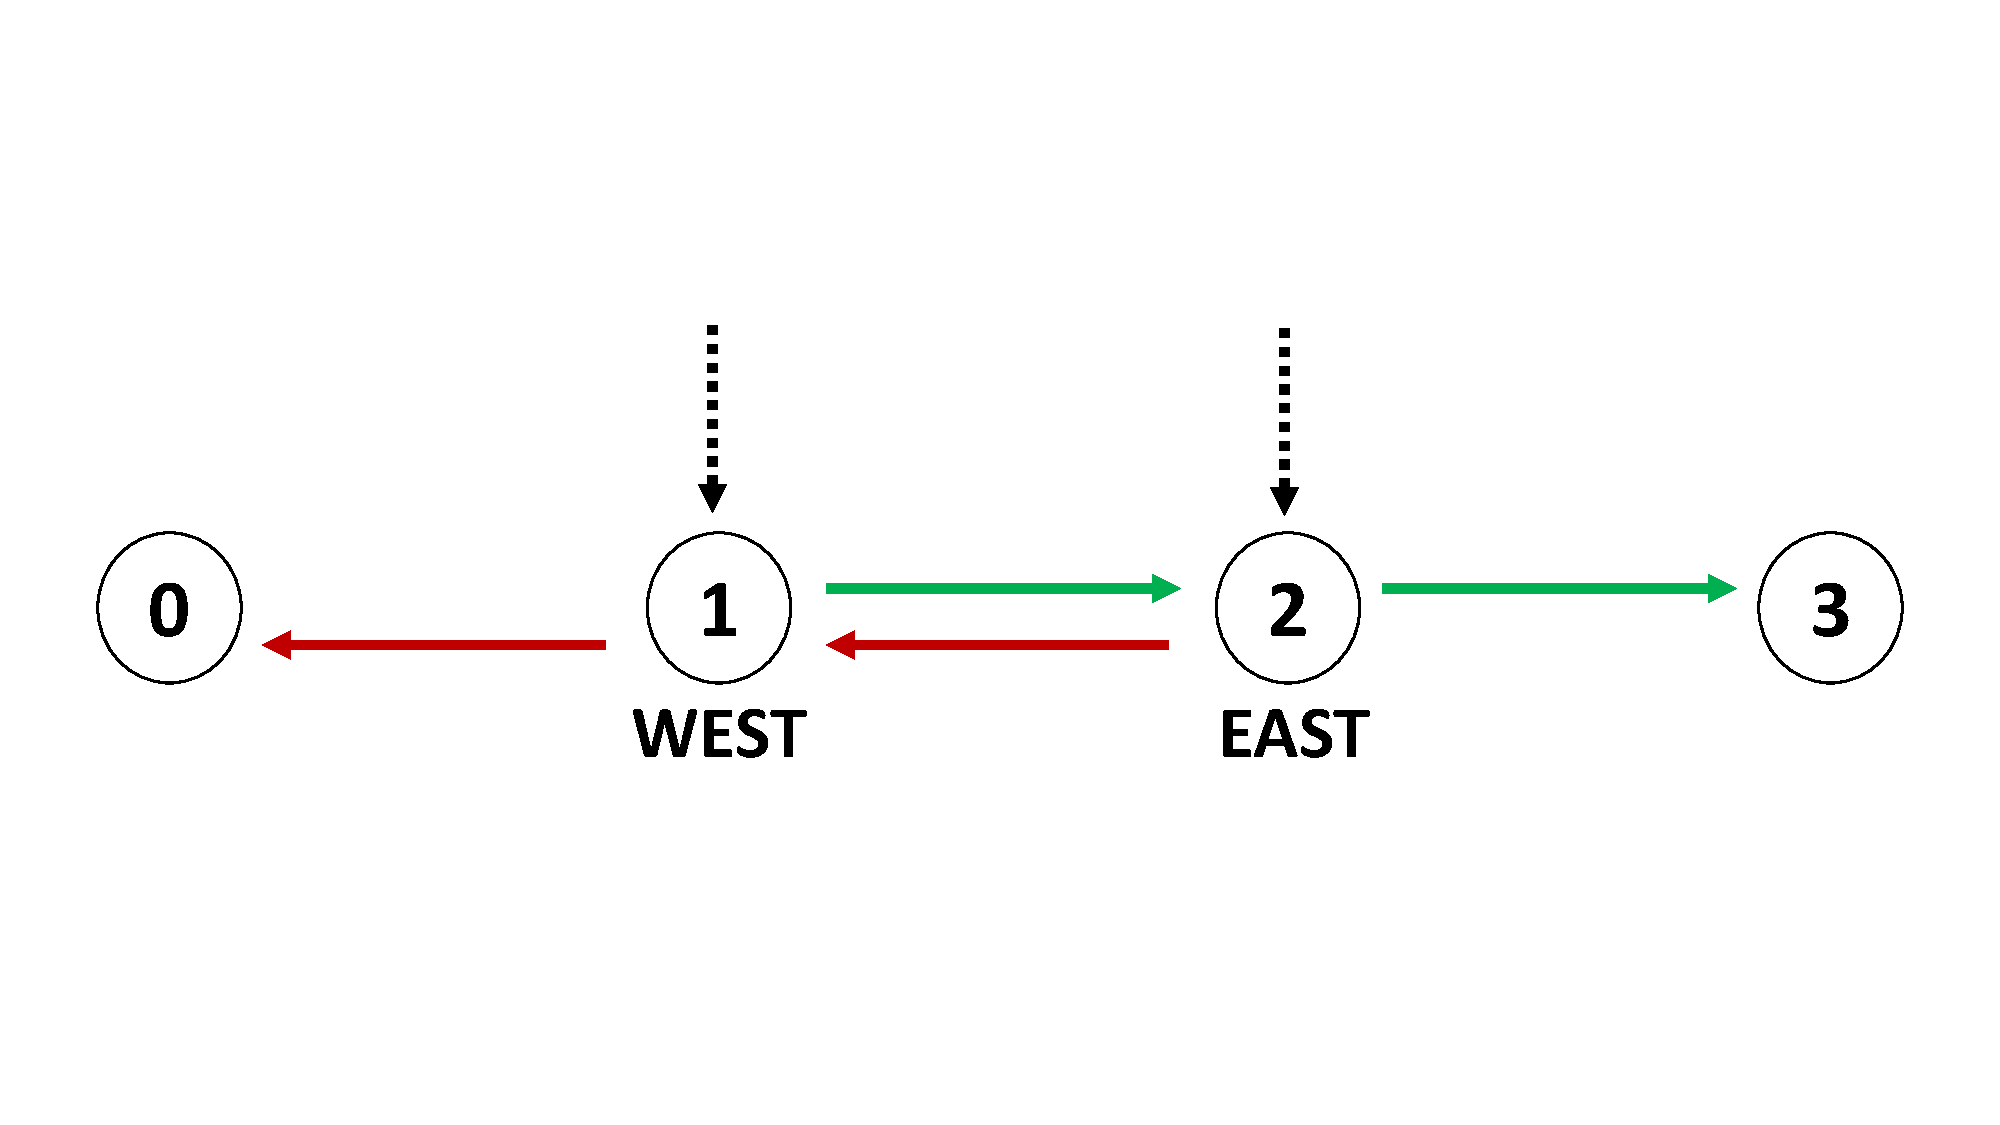
\includegraphics[width=0.65\linewidth]{plots/BgpColoredRouting.pdf}
%	\caption{Routing policy in example 7.}
%	\label{fig:pdfimage}
%\end{figure}

%\newpage
%
%
%example – 8
%
%\noindent
%\begin{minipage}[t]{0.45\textwidth}
%	\begin{lstlisting}[caption={foo (serializable)}]
%	request foo: 
%	    if (?):
%	        X := (X + 2) % 3 
%	        // no yield
%	        return X
%	
%	    else:
%	        X := (X + 1) % 3
%	        // no yield
%	        return X
%		\end{lstlisting}
%\end{minipage}
%\hfill
%\begin{minipage}[t]{0.45\textwidth}
%\begin{lstlisting}[caption={foo (non serializable)}]
%request foo: 
%     if (?):
%         X := (X + 2) % 3 
%         yield
%         return X
%
%     else:
%         X := (X + 1) % 3
%         yield
%         return X
%	\end{lstlisting}
%\end{minipage}
%
%One output that is attainable only via non-serializable executions is 
%\[
%\{(foo,1),(foo,1),(foo,1),(foo,3)\}
%\]
%
%
%%\newpage
%
%
%example – 9
%
%\noindent
%\begin{minipage}[t]{0.45\textwidth}
%	\begin{lstlisting}[caption={foo (serializable)}]
%request foo:
%    if(STOP == 0):
%        X := (X + 1) % 4
%
%    yield
%
%    if(STOP == 0):
%        X := (X + 1) % 4
%
%        STOP := ?
%        
%        if(STOP == 1):
%	        return X
%        return 0
%	\end{lstlisting}
%\end{minipage}
%\hfill
%\begin{minipage}[t]{0.45\textwidth}
%	\begin{lstlisting}[caption={foo (non serializable)}]
%request foo:
%    if(STOP == 0):
%        X := (X + 1) % 4
%
%    yield
%
%    if(STOP == 0):
%        X := (X + 2) % 4
%
%        STOP := ?
%        
%        if(STOP == 1):
%	        return X
%        return 0
%	\end{lstlisting}
%\end{minipage}


